

\documentclass[12pt]{article}
\usepackage[T1]{fontenc}
\usepackage[utf8]{inputenc}
\usepackage{amsmath}
\usepackage{microtype}
\usepackage{listings}
\setlength{\parindent}{0pt}
\usepackage{fancyvrb}
\usepackage{enumerate}
\usepackage{array}
\usepackage[breaklinks=true,linktocpage,hidelinks]{hyperref}
\usepackage[letterpaper]{geometry}
\usepackage{url}
\usepackage{graphicx}
\usepackage{fullpage}

\usepackage{pgfplots}
\usepackage{pgfplotstable}
\usepackage{tikz}

\usepackage{fancyhdr}
\usepackage{fancybox}
\usepackage{multicol}
\usepackage{xcolor}
\usepackage{adjustbox}

\pgfplotsset{compat=newest}
\usetikzlibrary{shapes,backgrounds,arrows}
\usepgfplotslibrary{external} 

\definecolor{brewcol1}{RGB}{166,206,227}
\definecolor{brewcol2}{RGB}{31,120,180}
\definecolor{brewcol3}{RGB}{178,223,138}
\definecolor{brewcol4}{RGB}{51,160,44}
\definecolor{brewcol5}{RGB}{251,154,153}
\definecolor{brewcol6}{RGB}{227,26,28}
\definecolor{brewcol7}{RGB}{237,179,1}
\definecolor{brewcol8}{RGB}{202,178,214}
\definecolor{brewcol9}{RGB}{206,27,1}

\geometry{hmargin=1.87cm, vmargin=1.87cm}
\bibliographystyle{siam}

\DeclareTextFontCommand{\helvetica}{\fontfamily{phv}\selectfont\small}


\begin{document}

\clearpage\thispagestyle{empty}
\begin{center}
\textbf{Difficult transition for sugar maple in Boreal forest under climate change? \\
Impact of alternative stable states on Sugar maple migration.}
\vskip 2em
Research proposal
\vskip 1em
Master in Wildlife management
\vfill
By
\vfill
Steve Vissault 
\vfill 
For
\vfill
\textbf{Richard Cloutier}, Pr.\\
Director of the program committee
\vskip 2em
\textbf{Dominique Arsenault}, Pr.\\
President of the jury
\vskip 2em
\textbf{Matt Talluto}, PhD\\
Research Co-director
\vskip 2em
\textbf{Dominique Gravel}, Pr.\\
Research Director
\vfill
\vfill
Université du Québec à Rimouski\\
\today

\end{center}

\newpage
\setcounter{page}{1}

\section{Introduction}

\textbf{Context.} Sugar maple (\textit{Acer saccharum}) is a widespread and
abundant tree species in north-eastern North America.
\cite{Graignic2013,Messaoud2007,Kellman2004,Barras1998}. Predicting shifts of
the range of Sugar maple is of prime importance because this species is highly
desirable for hardwood and maple syrup production, two large economic sectors
in Quebec. This species is dominating the temperate forest up to the boreal-
temperate  ecotone at its northern range limit \cite{Barras1998}. Some
representative species of northern forest ecosystems are expected to expand
their distribution towards the north following climate warming
\cite{Sciences2014,Iverson2002}. According to McKenney (2007)
\cite{Sciences2014}, the climatic conditions  favorable to Sugar maple  will
reach the Ungava bay within the next 100 years, which appears highly
improbable because of dispersal limitations and slow population dynamics. This
prediction relies on a species distribution model accounting only for climatic
conditions; it is recognized that Sugar maple regeneration depends both on
macro  (\textit{i.e.} regional climate) and micro environmental conditions
(\textit{i.e.} soil and microtopography) \cite{Graignic2013,Lafleur2010}. De
Frenne \textit{et al.} (2013) revealed that shifts in species distribution in
reaction to climate change can be mitigated by the microconditions (i.e. soil
temperature within the forest understory) rather than the macroconditions (i.e
temperature rising at regional scale). Hence, we anticipate that the
microconditions could also delay future sugar maple establishement into the
boreal forest.\\

Soil-plant feedbacks are susceptible to impact sugar maple migration dynamics.
Soil properties found in boreal forests differ from those in temperate forest
\cite{Lafleur2010,Barras1998,Goldblum2010,Demers1998}. A deep and poorly-
decomposed   litter layer is usually found in boreal forests, while the litter
of  northern hardwood forests is thinner and mainly composed of a superficial
leaf mat \cite{Barras1998}. The temperature is colder, the snow melts later
and the soil is wetter under coniforous trees \cite{Lafleur2010,Goldblum2010}.
Acid soils in coniferous forests causes a reduction in the cation exchange
capacity and subsequently decreases availability of some nutrients such as
calcium \cite{Moore2008}. Sugar maple seedlings have been recognized to be
particularly sensitive to waterlogged conditions and soil nutrient content
\cite{Moore2008,Lafleur2010,Cleavitt2011}. These properties of coniferous
forest soils could hinder the local establishment of species associated with
alkaline soils or unable to withstand waterlogged conditions
\cite{Lafleur2010}. Migration of temperate tree species therefore likely to be
restricted or delayed by the dominance of coniferous trees \cite{Lafleur2010}.
Thus, even if the climatic conditions at the regional scale become favorable
to Sugar maple after climate warming, the micro conditions found in the boreal
forest could slow seedling establishment
\cite{Kellman2004,Moore2008,Barras1998,Messier2011}. Sugar maple could thus be
unable to colonize the boreal forests as a result of strong and localized
soil-plant feedbacks \cite{McCarthyNeumann2012}.\\

My general hypothesis that the temperate-boreal forest ecotone is as a system
dominated by two alternative states, \textit{i.e.} contrasted equilibrium
states occurring under the same climate conditions
\cite{scheffer2009critical}: the boreal community and the temperate community,
including Sugar maple. Under this hypothesis, the landscape would be a patch
mosaic where micro conditions and stand history are driving the spatial
occurrence of boreal and temperate communities, despite a regional climate
favourable to temperate species \cite{Goldblum2010,Fisichelli2013}. I expect
that a climate warming and the subsequent incapacity of Sugar maple to
colonize boreal forest stands will create  tension between the potential and
realized forest composition and consequently that abrupt shifts in community
composition are susceptible to occur at the boreal-temperate forest ecotone.\\

\textbf{Objectives.} The main objective of this project is to investigate the
role of alternative stable states in the transition between the boreal and temperate
forests under different climate change scenarios. In this context, we will
test two specific hypotheses: ($H_1$) Alternative stable states do co-occur at
the boreal-temperate forests ecotone, and ($H_2$) the response of Sugar maple
to climate change will be delayed in areas where alternative stable states are
susceptible to occur. In order to fulfill this objective and test these
hypotheses, we will (1) develop a climate-dependent state-transition model
(STM) representing the dynamics of the boreal and temperate communities at the
landscape scale; (2) study the occurrence of alternative stable states at the
temperate-boreal ecotone; and finally (3) run simulations of the temperate
community species distribution under different climate change scenarios. The
first section of this proposal reviews the context of the study. I present
the concept of alternative stable states and critical transitions in forest
ecosystem properties. Then after I focus on Sugar maple, its associated
community in the temperate biome, and a justification about why alternative
stable states are expected to occur at the boreal-temperate forests ecotone.
The last section of this proposal describes the model and the methodology that
we will employ to achieve the specific objectives.

\section{Review} 

\textbf{Alternative stable states.} A community is stable when it persists in a
given state and is resilient to small perturbations \cite{Filbee-Dexter2013}. 
Multiple stables states are however possible for a single system. The idea that alternative
stable states may exist in community ecology was proposed in the late 1960s
\cite{Scheffer2001,Society2014a}.  May (1977) \cite{May1977} shown that an
ecosystem can be seen as a dynamic system where communities are not constant
over time and can change following a modification of the environnement.
Ecological communities can reach several equilibrium points 
along an environmental gradient \cite{May1977}. Stable states can persist
according to various feedback mechanisms \cite{Filbee-Dexter2013}. For
instance, in the Sahel or some part of the Amazone area, vegetation may
promote precipitation (i.e. positive feedback) and thus the persistence of
large tracts of forests. However, loss of vegetation  in this region following
logging or natural fires can lead to a major change in climate, which becomes
eventually too dry to support the vegetation needed to maintain precipitations
\cite{scheffer2009critical}. Hence, larger perturbations encountered by the
system can generate a change of the state of a community, i.e. the arrangement
of species or populations and their interaction with the physical environment
\cite {Filbee-Dexter2013}.\\

There are three possible responses of communities to a permanent
change in the environment: \textbf{(A)} gradual, \textbf{(B)} basic fold,
\textbf{(C}) catastrophic fold \cite{Scheffer2001} (Figure \ref{fig1}, upper
line). First, when a small modification on environmental condition occurs (e.g,
temperature rises), the state of the community can change almost linearly
(Figure \ref{fig1}.A) \cite{Scheffer2001,Scheffer2009}. In this case, the whole
ecosystem can be seen as a continuum of communities along the environmental
gradient \cite{Scheffer2001,Scheffer2009,scheffer2009critical}. Secondly, the
entire community can be insensitive to changing environmental conditions over a
certain range, but respond strongly when a threshold is reached
\cite{scheffer2009critical}. For instance, some species mortality can increased
sharply when a toxin is added to the environment and a lethal treshold is
reached \cite{scheffer2009critical}. In this case, the response curve of this
natural systeme is not linear but lightly folded. Hence, a small change of the
environment such adding a toxin, can lead to major changes in the  community
state. Lastly, in some strong non-linear systems, the response can be folded
backwards and alternative stable states could occur (Figure \ref{fig1} .C). This
implies that, for a given environnement, the ecosystem has two alternative
stable states ($F_1$ and $F_2$) separated by an unstable equilibrium (yellow
zone, figure \ref{fig1} .C). When the system approaches a tipping point on the
folded upper branch, it cannot pass smoothly to the lower branch. Small forcing
on initial conditions of the state $F_1$ transfers the system immediately to a
different state $F_2$ (Figure \ref{fig1} .C). At this point, the system is
particularly sensitive to the initial conditions. This point is called a
bifurcation point and a small forcing can drive the system into backward or
forward shifts towards either one of the alternative stable states $F_1$ or
$F_2$, also called "attractors" \cite{scheffer2009critical}. \\

The main ingredient to create alternative stable states is the occurrence of
positive feedbacks \cite{scheffer2009critical,Schroder2005}. One well known is
the facilitation process in ecology and two kinds exist in nature. The first
one is interspecific facilitation and can be observed across the ecological
succession process. Pioneer species pave the way for later successional
species, changing gradually the environment (e.g. shading, deeper litter)
\cite{scheffer2009critical, Levine2006}. In this case, the environmental
modification by pioneer species can be seen as a positive feedback allowing
the establishment of late successional ones.  The second kind of facilitation
is intraspecific, where a particular species can promote its own regeneration
in the immediate environment. \textit{Acer saccharum} and \textit{Tsuga
canadensis} seedling establishement for instance is impacted by the unique
seedbed conditions created by each species, promoting self-replacement
\cite{Society2014,McCarthyNeumann2012}. By changing seebed conditions, mature
trees promote their own regeneration,. When the intraspecific facilitation is
higher than the interspecific competition, we can observed forest stand
dominated by mature trees of \textit{Acer saccharum} and else by \textit{Tsuga
canadensis}. Hence, either forest stand type can be considered as an
alternative stable state. This kind of positive feedback is susceptible to
occur at the boreal-temperate forest ecotone we will study
\cite{Barras1998,Society2014}. \\

\begin{figure}[t]
	\begin{center}
	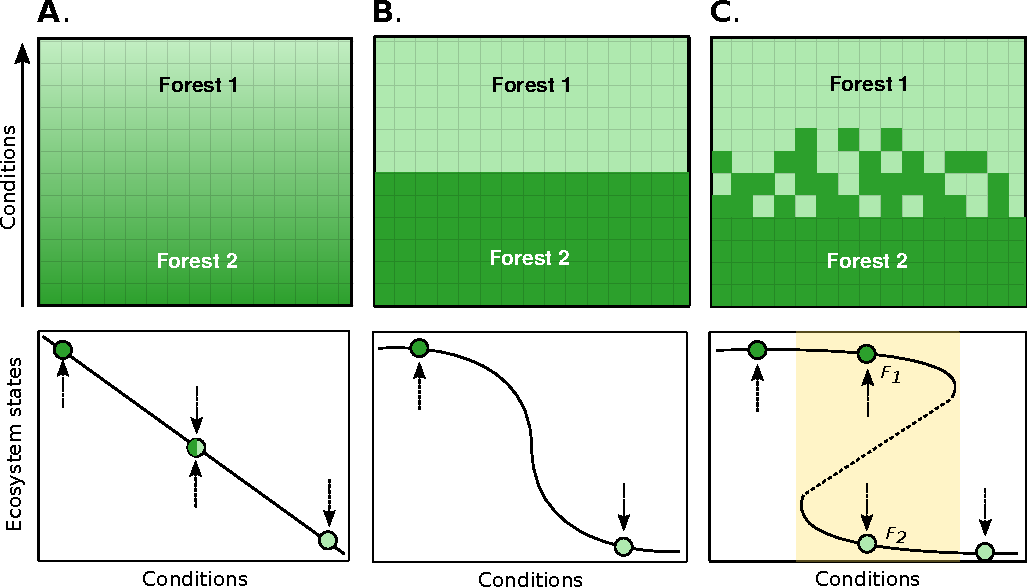
\includegraphics[width=0.8\textwidth]{fig/states.pdf}
	\end{center}
	\caption{Change in communities composition over an environmental gradient (i.e. precipitation, temperature or soil moisture) can take three different shapes: \textbf{(A)} gradual, \textbf{(B)} basic fold,
	\textbf{(C}) catastrophic fold. Each of them are shown across the upper
	line. Solid lines represent all reachable stable states along the climate gradient.  Arrows indicate
	where the system moves if not at the equilibrium (i.e outside of the solid lines). The yellow zone (in panel C),
	called hysteresis, is unstable and small fluctuations onto the environment
	conditions could give rise to abrupt changes into one of the alternative
	stable states ($F_1$ or $F_2$). In the temperate-boreal system and according to each response shape, the bottom line illustrate three different spatial repartitions of boreal and temperate communities over a climatic gradient.}
	\label{fig1}
	\vspace{-1em}
\end{figure}


\textbf{Natural system studied.} Many empirical and modelling studies have
been conducted on the transition between forest to non-forest communities
(e.g. Boreal-Tundra) \cite{Scheffer2012,Scheffer2001,Hirota2011,Messaoud2007}.
However, little attention has been given to understand the forest-forest
ecotone's dynamic \cite{Goldblum2010,Graignic2013,Messaoud2007}.  The
temperate-boreal transition could adopt three different structures along a
climatic gradient (Figure \ref{fig1}, lower line). In the first case, the
response of forest communities to climate is gradual and no disctinct boundary
is observed between the temperate and the boreal forests (Figure
\ref{fig1}.A). Instead, a smooth transition occurs along a climatic gradient.
On the other hand, distribution of temperate and boreal forest communities can
be strongly linked to climate. Thus, climate highly segregate forest types and
a net boundary appears between them (Figure\ref{fig1}.B).  Finally, a third
response  of the system is also possible. Previous studies highlighted that a
broad zone in the boreal- temperate forests transition exists where stands
dominated by either coniferous or deciduous species co-occur at the regional
scale, but not within stands \cite{Goldblum2010,Fisichelli2013}. Hence, this
spatial configuration might correspond to the third case shown in figure 1.C.
We hypothesize these communities to be alternative stable states. A strong
positive plant-soil feedback might contribute to the maintenance of these
communities: coniferous species generate acidic and wetter soils and deciduous
species enrich the litter. Both types of forest stands are facilitating their
own regeneration.   These feedbacks help temperate species seedling
establishement in favorable sites of an heterogeneous landscape.\\

Positive feedbacks should not increase the growth rate of temperate species
within patches they already dominate, but they should increase local density
and seed production \cite{Levine2006}. A large disturbance could however
contribute to modify the microconditions in a patch historically unfavorable
to the other species. Following this event, this disturbed patch can switch
abruptly into a temperate forest if fa seed source is present in the
neighborhood. These feedbacks might influence the spreading rate of temperate
species into boreal forest \cite{Levine2006}. In unfavorable patches,
temperate species will have to cope with boreal soil properties that may
hinder and delay their establishment. Climate change also has the potential to
improve boreal soil conditions for temperate species establishment
\cite{Lafleur2010}. The outcome of these antagonistic forces could impact
postively or negatively the migration of some temperate species in response to
climate change.

\section{Methods}   

\textbf{State and Transitional Model.} This study will be based on a STM
representing landscape dynamics at the boreal-temperate transition. Three
forest cover types are considered: (i) deciduous, (ii) mixed and (iii)
coniferous \cite{Fisichelli2013}.  Each of these stand types is represented as
a state in the STM: \textbf{(D)} Deciduous, \textbf{(M)} Mixed, \textbf{(C)}
Coniferous. We also consider the state \textbf{(T)} to represent transitional
stands (green circles, figure \ref{Model}).  According to Briske\textit{ et
al.} (2008), a state means a plant community phase occurring on similar soils
that interact with the environment to produce persistent functional and
structural attributes. Transition between states are climate-dependant.
Transitions between all states are possible except the direct transition
between a deciduous and coniferous stand, which requires an intermediate step
through state M. Except for the colonization probability ($\theta$),
transition probabilities vary with the proportion of coniferous or deciduous
found in the  neighbourhood to represent dispersal limitations. For instance,
the succession rate of a coniferous patch ($\beta_c$) towards a mixed patch
(M) depends also on the availability of D and M patches in the landscape
(figure \ref{Model}).  \\

\begin{wrapfigure}{L}{0.45\textwidth}
	
\begin{center}
	
				\tikzstyle{noeud}=[circle,
				                  thick,
				                  minimum size = 1.5cm,
				                  inner sep =5pt,
				                  draw=brewforest3,
				                  fill=brewforest1]
				\tikzstyle{noeud2}=[circle,
				                  thick,
				                  minimum size = 1.5cm,
				                  inner sep =5pt,
				                  draw=brewforest3,
				                  fill=brewforest3]
				\tikzstyle{noeud3}=[circle,
				                  thick,
				                  minimum size = 1.5cm,
				                  inner sep =5pt,
				                  draw=brewforest3,
				                  fill=brewforest3]
	
				\begin{tikzpicture}[->,>=stealth',auto,scale=0.65]
				      \node [circle,noeud2] (M) at (0,0) {\color{white}\textbf{M}};
				      \node [circle,noeud2]  (C) at (-5,5) {\color{white}\textbf{C}};
				      \node [circle,noeud2] (D) at (5,5) {\color{white}\textbf{D}};
				      \node [circle,noeud2] (T) at (0,10) {\color{white}\textbf{T}};
	
						\draw[thick,-latex] (M) to[bend right=10] node[above,sloped] {$S_C$} (C);
						\draw[thick,-latex] (C) to[bend right=10] node[below,sloped] {$\beta_d \cdot (D+M)$} (M);
	
						\draw[thick,-latex] (D) to[bend right=10] node[above,sloped] {$\beta_c \cdot (C+M)$} (M);
						\draw[thick,-latex] (M) to[bend right=10] node[below,sloped] {$S_D$} (D);
	
						\draw[thick,-latex] (D) to[bend right=10] node[above,sloped] {$e$} (T);
						\draw[thick,-latex] (T) to[bend right=10] node[below,sloped] {$\phi_D$} (D);
	
						\draw[thick,-latex] (T) to[bend right=10] node[above,sloped] {$\phi_C$} (C);
						\draw[thick,-latex] (C) to[bend right=10] node[below,sloped] {$e$} (T);
	
						\draw[thick,-latex,transform canvas={xshift=0.8ex}] (T) to node[above,sloped,rotate=90,transform canvas={xshift=3ex}] {$\phi_M $} (M);
						\draw[thick,-latex,transform canvas={xshift=-0.8ex}] (M) to node[above,sloped,rotate=-90,transform canvas={xshift=-3ex}] {$e$} (T);
				\end{tikzpicture}
	\end{center}	


	\caption{Conceptual representation of the transition model between deciduous ($D$),
	mixed ($M$) and coniferous ($C$) stands. $T$ corresponds to a post-disturbance forest stand. Perturbations, natural and anthropogenic, occur with a probability $\epsilon$. 
	Flows or transition rates between states are represented by arrows.
	Parameters $\theta$ and $\beta$ are  colonization and succession probabilities,
	respectively. We define regeneration functions $\phi_c$ , $\phi_d$ as $\phi_c
	= \alpha_c \cdot (M+C) \cdot [1- \alpha_d \cdot (D+M)]$ and $\phi_d =
	\alpha_d \cdot (D+M) \cdot [1- \alpha_c \cdot (C+M)]$. $\phi_m$ include these both equations giving $\phi_m = \phi_c \cdot \phi_d$. Finally, parameter $\alpha$ represents the climate-dependent regeneration rate after a patch has been disturbed.}
	\label{Model}
	\vspace{1em}
\end{wrapfigure}

Ecological processes such as succession and colonization are not the only
mecanisms responsible for the transition between two states. Natural
disturbances are important drivers of forest dynamics at the landscape scale
(e.g. fire in boreal forest or large windthrow in temperate forest). Small
fires promote dominance by deciduous species, while larger and intense fires
favour boreal communities \cite{Bergeron2004}. Anthropogenic disturbances such
as logging can also produce major change in the forest composition. Dupuis
\textit{et al.} (2011) revealed that historical disturbances affected the
expansion (maples/aspen) or decline (cedar/spruce) of several species at the
northern range limit of temperate trees in eastern Québec \cite{Dupuis2011}.
When a disturbance occurs in the actual model, the state affected is
systematically converted into a transitional state \textbf{(T)}. (Figure
\ref{Model}).  Then after, any transitional patch (\textbf{T}) can switch into
state C, M or D according to a probability $\phi$. In the conversion case of
state T towards C,

%DG: ce n'est pas un flow, mais une probabilité. Un ensemble très grand de probabilités devient un flux (parce que la variance diminue), mais pour ça il faut changer d'approche conceptuelle du modèle; pour l'instant, tiens toi à un modèle stochastique)

this flow $\phi_c$ incorporates a specific patch regeneration rate
($\alpha_c$), as well as the availability of coniferous $(C + M)$ species and
the proportion of patches unconverted into a deciduous state, $1- \alpha_d
\cdot (D + M)$ (see caption, figure \ref{Model}). If this patch $C$ is
undisturbed, then it could switch to a mixed stand after colonization by
deciduous trees with a probability $\theta_c$. The dynamics of a large number
of patches following these rules can be described with a system of four
differential equations. The dynamics of $T$ over the time is described by the
following differential equation:

\begin{equation}
 	\frac{\delta T}{\delta t} =\epsilon \cdot (C+M+D) - T \cdot (\phi_d + \phi_c + \phi_m)
\end{equation}

The differential equations illustrating the dynamics of the other three states
(C, M and D) in the system are relatively similar and can be described (with
coniferous state as example):

\begin{equation}
	\frac{\delta C}{\delta t} = \phi_c \cdot T + \theta_c \cdot M -\alpha_d \cdot (D+M)\cdot C - \epsilon \cdot C
\end{equation}

This model is spatially implicit and assumes that each patch is occupied by
one state, thus the proportion of all states sum to 1. \\

\textbf{Data description.} The parameterization and validation of the model
will be conducted using the QUICC- FOR\footnote{Quantifying and mapping impact
of climate change on the forest productivity in eastern Canada.} database of
permanent (PP) and temporary (TP) sample plots from United States and Canada.
The data has been freely provided by partners and covers 3 eastern Canadian
provinces (\textit{ca.} 16,000 plots) and 31 states of eastern USA
(\textit{ca.} 150,000 plots). Surveys started in the 1970s and include up to 5
remeasurements, with the interval between sampling ranging from 5 to 10 years.
Data is recorded for seedlings, trees, saplings and stand level. Stem-level
information includes diameter at breast height (DBH), species, state of the
stem (e. g. alive or dead), height, age and canopy position. Seedling and
sapling data provide numbers of individuals by class of DBH and species. The
stand-level data includes relevant information about soil deposit, drainage,
disturbances, cover type and age and height of the stand. All  inventories are
geo-referenced. Climatic variables are associated to each plot by
interpolating  the climatic model ANUSPLIN \cite{McKenney2011} . We will
parameterize the model using annual rainfall (mm) and monthly temperatures
(minimum, maximum and average in \ensuremath{^\circ}C) of the 30 years
previous to the year of each plot's sampling. Those variables are used by many
authors as good predictors of the distribution of the species investigated in
this present study \cite{Goldblum2010}. Filters will be applied to the
database prior to the model parameterization. As a first step, out of the 57
species contained in the database, only 28 representative species of the whole
dataset will be taken into account. Only plots with mesic soil conditions,
\textit{i.e.}, thick deposits with fast to moderate drainage, will be
considered for the analysis. We will consider only mature stands with dominant
strata containing trees greater than 50 years old. Lastly, plots disturbed by
human activities (mostly by logging) will be removed in order to parametrize
the model using only natural disturbances. \\

\textbf{Parametrization.} The model focuses on representative species of the
boreal and temperate forest. Relative  abundance of each species will be
computed from basal area in each of the plots and at each time step (year of
measurement). Stands will be considered in one of the four states previously
described in the model section (Figure \ref{Model}). C, M, D and T states will
be classified following their percentage of $Ba$ in deciduous ($Ba_d$),
coniferous ($Ba_c$) or transition species ($Ba_t$) in the plot (Table
\ref{bound}). The plots that do not satisfy any of the conditions shown in
table \ref{bound} will be filtered out.\\

\begin{table}[h]
\vspace{-1em}
\centering
\caption{Boundary of the coniferous ($Ba_c$), deciduous ($Ba_d$) and transition species ($Ba_t$) relative abundances to classify the four STM's states (D,C,M and T). The symbol ($!$) means that the forest plot hasn't been previously classified into one of the states C, D or M.}
\vspace{-1em}
\small
\begin{tabular}{|l|l|}
	\hline
	\textbf{States}  & \textbf{Boundaries}                            \\
	\hline
	D & $Ba_c< 25\%$ and $Ba_d \geq 75\%$    \\
	C & $Ba_c \geq 75\%$ and $Ba_d < 25\%$    \\
	M & $Ba_c \geq 25\%$ and $Ba_d \geq 25\%$ \\
	T & $!D;!C;!M \text{ and }  Ba_t  \geq 75\%$ \\
	\hline                               
\end{tabular}

\label{bound}
\end{table}

The second step of the parameterization consists of evaluating functions
describing the probability of a transition between two states given specific
climatic conditions ($Climate$, eq. \ref{eq1}) and the proportion of deciduous
or coniferous in the neighborhood ($\hat{D}$ and $\hat{M}$, eq. \ref{eq1}).
Hereafter, will focus only on a specific transition $M \rightarrow T$ but the
method is common to  all transitions. In this example (eq. \ref{eq1}),
$\hat{D}$ and $\hat{M}$ are the expected probabilities of observing state D or
M in this area given climatic conditions. They are proxy for the deciduous
propagule pressure coming from neighbors. They will be estimated using  a
standard species distribution model (Step 1, eq. \ref{eq1}) such as the random
forest algorithm (R-package, \cite{Liaw2002a}).

\begin{equation}
	P(D_{t1}|M_{t0}, Climate) = f(\overbrace{Climate, \underbrace{\hat{D}, \hat{M}}_\text{Step 1. RandomForest}}^\text{ Step 2. Multinomial regression})
\label{eq1}
\end{equation}

The probability of a transition between two states given the local climatic
conditions encounter by a patch (Step 2, eq. \ref{eq1}) will be computed using
a multinomial regression (nnet R-package, \cite{Venables2002}). We can
summarize this multinomial regression as $P(D_{t1}|M_{t0}) \sim \hat{D} +
\hat{M} + X_1+X_2+X_i... $ where $\hat{D}$ and $\hat{M}$ correspond to the
probability of observing any state in the immediate neighbourhood (previously
presented) and $X_i$ a climate variable. Model selection will be performed
using Akaike's information criterion (AIC). The selected model will be used to
represent all transition probabilities between states.   \\

\textbf{Model validation and simulations.}  The model will be validated using
the temporary sample plots (TP), an independent dataset for the Québec
database. Temporary plots will be classified into the same four states. We
will compute the proportion of each state by ecoregion ("\textit{Système de
classification des types écologiques}", MRN) and compare this distribution to
the one predicted by the model.  Highest R-square and lowest Akaike
information criterion (AIC) will be associated with the best predictive and
parsimonious model.

%DG: bias is not a low r-square: it is a prediction that significanlty departs from the 1:1 relationship (e.g. over prediction of something, indicated by a positive intercept significanlty larer than 0)

Bias (i.e low R-square) might indicate that the current forest composition is
not at equilibrium and needing further investigations. After the validation,
we will assess if alternative stable states are present in the boreal-
temperate forests transitions ($H_1$). We will run multiple simulations of the
spatially implicit model in varying initial conditions i.e. states proportion
and climate conditions. In studying the simulations, we expect to find abrupt
changes in states proportion over the time. Also, we expect to oberved bimodal
distributions of states over a certain range of climate conditions (when the
model is at the equilibrium). If these expectations are validated then
alternative stable states are present in the boreal- temperate forests system.
In this spatially implicit model, rates of transition depend to the proportion
of states available in the general system, thus rates of transition are
unconditional to the state of patches in the neighborhood.

%DG: reword the previous sentence, and the following one

This property of the model makes it impossible to assess sugar maple range
schift (i.e. dispersal and velocity rates of forest temperate patches) as
proposed through hypothesis $H_2$. We will therefore simular this model over a
lattice (a cellular automaton), where each cell corresponds to a forest patch
in the landscape (C,D,M or T). The succession ($\beta$) and regeneration
($\alpha$) probabilities of transition will be positively affected by the
composition of the eight neighboring cells.  With this explicit model, we will
run simulations with a changinc climate (e.g. rise the temperature). We expect
to observed a rate of sugar maple migration strongly delayed or mitigated
where the alternative stable states appear.

%DG: dernier point, comment tu vas détecter ce délai?

\clearpage
\bibliography{/home/steve/Dropbox/Bibtex/Devis}
\end{document}